\documentclass[12pt]{article}

\usepackage[english]{babel}
\usepackage[utf8x]{inputenc}
\usepackage{pdfpages}
\usepackage{lastpage} % Required to determine the last page for the footer
\usepackage{extramarks} % Required for headers and footers
\usepackage{graphicx} % Required to insert images
\usepackage{listings} % Required for insertion of code
\usepackage{courier} % Required for the courier font
\usepackage{placeins} % Required to specify float barriers
\usepackage{caption} % Required for table captions

% Margins
\topmargin=-0.45in
\evensidemargin=0in
\oddsidemargin=0in
\textwidth=6.5in
\textheight=9.0in
\headsep=0.25in

\linespread{1.1} % Line spacing

\newcommand{\Title}{CSIR - Mobile Augmented Reality Number Plate Recognition} % Project Name
\newcommand{\Class}{Requirements\ Specification} % Doc Title
\makeatletter
%\renewcommand{\section}{\@startsection
  % {section}%                         name
  % {1}%                               level
  % {0mm}%                             indent
  % {-1.5\baselineskip}%               space above header
   %{0.5\baselineskip}%                space under header
  % {\sffamily\bfseries\upshape\normalsize}}% style
%\renewcommand{\subsection}{\@startsection
 %  {subsection}%                      name
 %  {2}%                               level
 %  {0mm}%                             indent
 %  {-0.75\baselineskip}%              space above header
 %  {0.25\baselineskip}%               space under header
 %  {\rmfamily\normalfont\upshape\normalsize}}% style
%\renewcommand{\subsubsection}{\@startsection
%   {subsubsection}%                    name
%   {3}%                               level
%   {0mm}%                             indent
%   {-0.75\baselineskip}%              space above header
%   {0.25\baselineskip}%               space under header
%   {\rmfamily\normalfont\slshape\normalsize}}% style
%\makeatother


\begin{document}

        \vspace{4em}
        
        \begin{center}%
        
          \LARGE \bf \Title \\[4em]
          \LARGE {\bf Architecture Specification Proposal}\\[1em]
          \LARGE {\bf Team Members:}\\[2em]
          \large
          
             Mbulungo Musetsho                          (10176382)  \\[1em]
             Ndivhuwo Nthambeleni 						(10001183)	\\[1em]
             Joas Mogale 								(10354167)	\\[1em]
                %Enter your details below just as the one above
            
        \end{center}%
        \begin{figure}[h]
	           \centering
	           
\includegraphics[width=1.27in, height=1.09in]{Pictures/csir.png}
	   	\end{figure}
	    \FloatBarrier
        

        \newpage
        \tableofcontents    
                \newpage
                \section{Introduction}
                		This document contains a detailed specification how the augmented reality project is going to be carried out by the Gruners group. It will specify both functional and non-functional requirements and the architectural design for the system. All these will be coupled with use cases for each particular system functionality and the testing thereof. This document will use agile methodologies to promote adaptation of the process to possible requirements changes and many other amendments based on practical issues that will be encountered throughout the process. 
               	%input
                \section{Vision and Scope}
                		\subsection{Vision}
                				The vision of the project is to develop a mobile application for smart phones that will enable the phone to detect vehicle number plates using a camera view and then access, from the display, the information of the scanned vehicle in real-time. This application will then be used by mobile units to track vehicle statuses. For instance, whether the vehicle was stolen or not road-worthy.
                		\subsection{Scope}
                			
                				The envisioned system is a mobile application, with a web front-end, which will allow the permitted users to do the following:
                			    		\begin{itemize}
                								\item scan through number plates for detection with the mobile application
                				                \item view the resulting information per detection in a user-friendly display.
                				                \item make all relavent CRUD operations, using a user-friendly web interface.
                				                
                			            \end{itemize}
                			            
           						\begin{figure}[h]
			           				\centering
			           				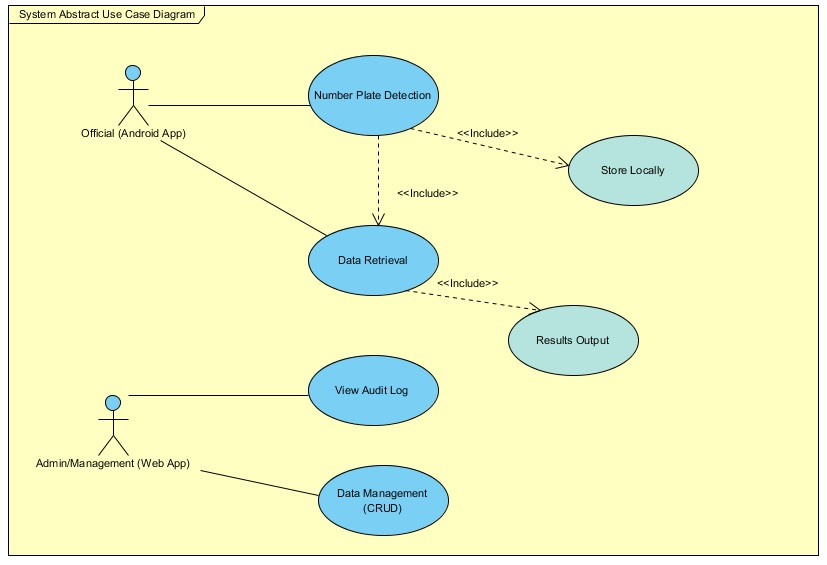
\includegraphics[width=5.51in, height=3.77in]{Pictures/AbstractUseCase.jpg}
			           				\caption{Abstract System Use Case Diagram}
           						\end{figure}
                				\FloatBarrier
                				
                \section{Architectural Requirements Specification}
                		\subsection{Access Channels }
                				The envisioned system must be accessible by human users via the Android application (for number plate detections) and Web browsers (for management activities).
                			
                		\subsection{Quality Requirements}
                		
                				\subsubsection{Performance}
		   			                  	The system must offer fast performance in detection of vehicle number plates as well as retrievals from the database. 
		   			                  	
                			    \subsubsection{Accuracy}
                			    		All detections must be verified for accuracy before the detection process continues.
                			    		             	
                				\subsubsection{Auditability}
		   			                   	The system must maintain audits for all vital operations. These audit logs can then be provided upon request. 
		   			            		
		   			            		
                				\subsubsection{Scalability}
	   			                   		The system must allow multiple users to make use of the application without interruptions. This holds for both the Android application and the web application.
		       			                  	
               					\subsubsection{Maintainability}
					                  	All layers of the system must be developer-friendly. - That is, the design and development of the system must allow smooth maintenance of all the system's counterparts.
       						    
       						    \subsubsection{Usability}
			    	                  	The system must allow all users to be able to interact with it without any major difficulties.
       						    	                  	
                
                		\subsection{Architecture Constraints}
                				
                				\begin{itemize}
                						\item The mobile application has to run on the Android OS with the target being Android 4.4 but allowing for compatibility with older versions up to Android 4.0.3. 
                						\item The MVC (Model View Controller) architecture pattern is to be used throughout the project.
                				\end{itemize}
               
                \section{Software Architecture Specification}
                
               		 \subsection{Architecture Requirements}
               		   
                			\subsubsection{Quality Requirements}
                					\begin{itemize}
                							\item Performance
	                								\begin{itemize}
						   			                  		\item Number plate detection must take less than 5 seconds from application start-up.
						   			                  		\item Retrieval of information from the database must take no longer than 1 second.
						   			                \end{itemize}
                								
                							\item Accuracy
			              							Number plate detections must be at least 99.99\% accurate. Detections made on non-stationary vehicles must be possible for vehicles at most 20 metres away from the scanning device.
               								
                							\item Auditability
		               								\begin{itemize}
		               									\item The system will make audits of all operations that alter the database.
		               									\item The system will also maintain a history of all number plate scans successfully done.
		               								\end{itemize}
		               								
		               								
                							\item Scalability
                									\begin{itemize}
					       				                  	\item The system must be able to scan all types of Southern African number plates.
					       				                  	\item The system must be able to operate effectively and efficiently under a load of 10000 concurrent android application users or 100 concurrent web interface users.
					       			                \end{itemize}
		               								
                							\item Maintainability
                									To implement maintainability, the system will make use of a layered architecture that separates certain counterparts such that maintaining a subsystem does not, in any means, affect any other subsystem.
		              								
                							\item Usability
                									An average user must be able to use the system without any further training or extensive manual consultation required. This will be achieved by the use of design principles to enhance user experience.
		               								
                							
                					\end{itemize} 
                			 
                			\subsubsection{Integration and Access Channel Requirements}
                					These are the different channels through which the system can be accessed by all related users.
	                				The system will be accessible by human users through the following channels:
	                				
			                    	\begin{enumerate}
					                    	\item From the web browser through a user-friendly web interface. This implies that the system must be accessible from all widely used web browsers (including the most recent versions of Mozilla Firefox, Google Chrome, Apple Safari and Microsoft Internet Explorer).
					                    	\item From mobile android devices using the Android application.
			                    	\end{enumerate}  
			                    	  
                			\subsubsection{Architecture Constraints}
                					The following architecture constraints will be followed mainly for maintainability reasons:
                					\begin{enumerate}
                							\item All system counterparts must be developed and attached to a JAVA RESTful Web Service.
                							\item The business logic layer must provide an API for access to the SQL Database.
                							\item The system will make use of a MySQL database.
                							\item The mobile client must run on an Android application.
                							\item The system functionality will be hidden in a RESTful web service such that it is not exposed to any presentation layer counterpart.
                					\end{enumerate}
                				
                			  
                	\subsection{Architectural patterns or Styles}
                			For the sake of good high-level responsibility separation and allowance for reuse of lower level layer components across components in higher level layers, a layered architecture will be used for this system.
                			The layered architecture for the system contains the following layers:
                			\begin{itemize}
		                			\item Client Layer
		                			\item Access Layer
		                			\item Business Processes Layer
		                			\item Domain Objects Layer
		                			\item Backend Layer
                			\end{itemize} 
                			
                			
                			\begin{figure}[h]
                                   \centering
                                   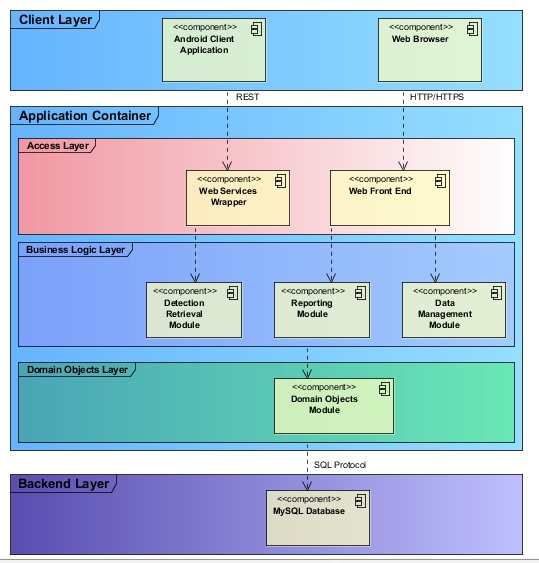
\includegraphics[width=3.59in, height=3.75in]{Pictures/SystemArchitectureLayers.jpg}
                                   \caption{System Layered Architecture}
        					\end{figure}
        					\FloatBarrier
                			
                			
                			The responsibility allocation across the layers is as follows:
                			\begin{enumerate}
                					\item Provide access to humans: Client Layer
                					\item Provide access to system functionality to human access layer and other systems: Access Layer
                					\item Business Logic Encapsulation: Business Processes Layer
                					\item Provide domain objects: Domain Objects Layer
                					\item Hosting Database: Backend Layer
                			\end{enumerate}
                			
                    % Commented out for later stage:\subsection{Architecture Tactics or Strategies}
                    % Commented out for later stage: \subsection{Use of Reference Architecture and Frameworks }
					\subsection{Technologies}
							Technologies that will be used throughout the system development include:
							\begin{itemize}
								\item JAVA Native Android SDK
								\item HTML 5
								\item JAVA Programming Language
								\item Qualcomm Vuforia Augmented Reallity SDK
								\item MySQL Database for JDBC
							\end{itemize}
                    
                \section{Functional requirements and application design}
                    \subsection{Introduction}
                    This section discusses all the functional requirements for the CSIR Augmented Reality Number Plate Recognition system.
                    
                    \subsection{Required functionality}
                    		\subsubsection{Number Plate Detection}
                    				Upon opening the application, it displays a real-time view of the android device's rear camera. Using Augmented Reality, an orange box is drawn around a detected number plate. There may be multiple number plates in a scene. At this stage the "Detection Local Storage" use case is triggered to store the scanned number plates locally, after which the "Data Retrieval" use case is triggered to fetch data from the server. If the plate is not found or OK, then the box around the plate turns green and an audible tone indicates the check is complete. If the database returns a bad result (stolen, outstanding ticket, etc.), then the box should turn red and a different tone should be sound.
                    				Clicking on a box will open the number plate details screen, displaying any additional information available.
                    				\begin{figure}[h]
					           				\centering
					           				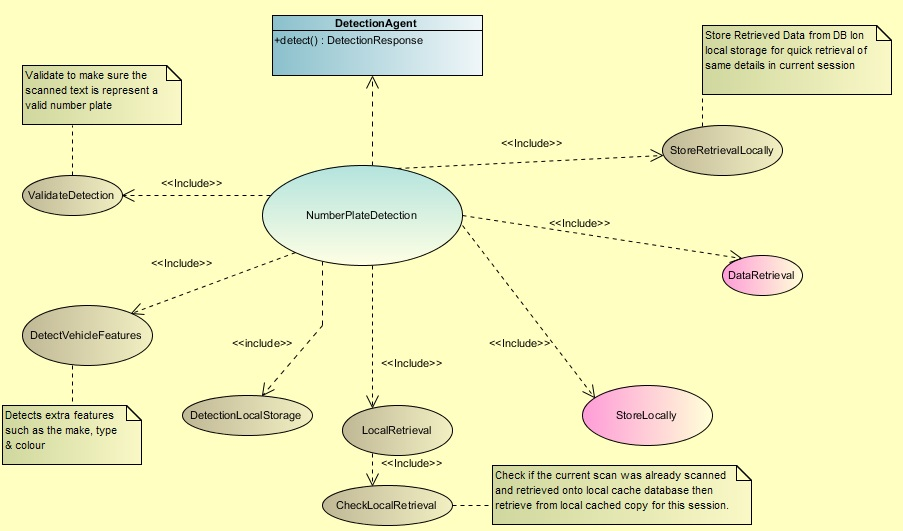
\includegraphics[width=6.25in, height=3.67in]{Pictures/NumberPlateDetectionUseCase.jpg}
					           				\caption{Number Plate Detection Use Case Diagram}
		           					\end{figure}
                    				\FloatBarrier
                    				
                    				\begin{figure}[h]
					           				\centering
					           				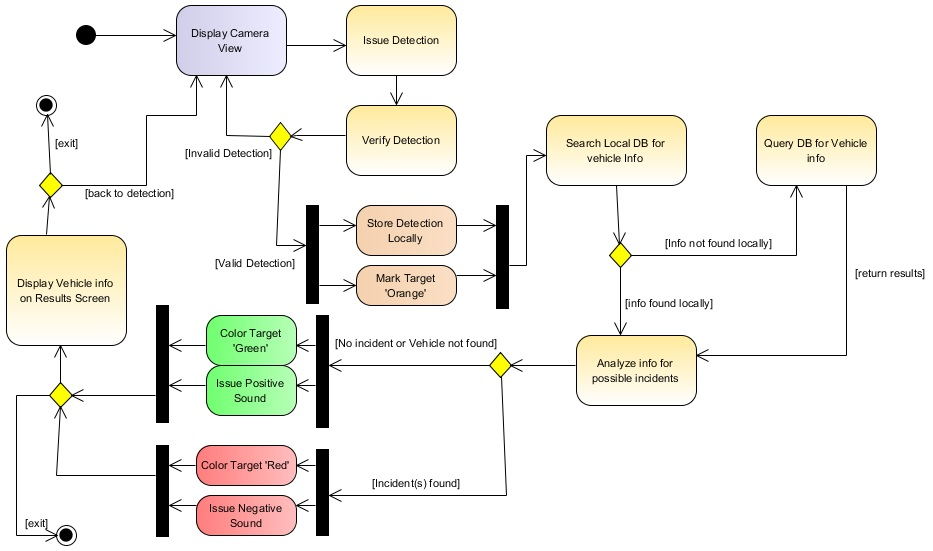
\includegraphics[width=6.25in, height=3.67in]{Pictures/NumberPlateDetectionActivity.jpg}
					           				\caption{Number Plate Detection Activity Diagram}
		           					\end{figure}
		                  				\FloatBarrier
                    				
                    		\subsubsection{Detection Local Storage}
                    				Once the mobile application has made a detection, this use case is triggered just before data is requested from the database. The system needs to keep record of all the scans the user has made. So the system will store the detected number plate string onto a local database. All other features detected with the number plate will be stored locally as well (e.g. colour, make, type, model).
                    				\begin{figure}[h]
					           				\centering
					           				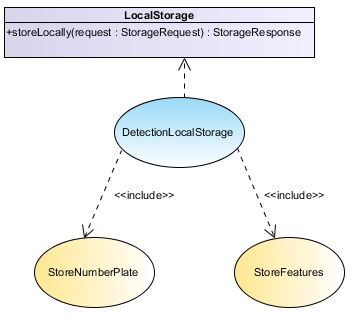
\includegraphics[width=2.5in, height=2.21in]{Pictures/DetectionLocalStorageUseCase.jpg}
					           				\caption{Detection Local Storage Use Case Diagram}
		           					\end{figure}
                    				\FloatBarrier
                    		\subsubsection{Data Retrieval}
                    				Data Retrieval may be triggered either by the user (via a searchable list of detected number plates stored locally) or by the system as a sequence of use cases. Its function is to retrieve information related to the requested number plate. Firstly, the application searches against its local database in case the information had already been retrieved in the current session. If there's no match, it makes an HTTP query to fetch data pertaining to a particular number plate. The retrieved data is stored onto the local database for display. This information is only kept locally per session. When the session is closed this storage is cleared to ensure that the next session retrieves the most recent data from the remote database.
                    		
                    		\subsubsection{Results Output}
                    				When the user clicks on a number plate that was detected (Either from the live camera view or from the list of scanned number plates stored locally), this function fetches the retrieved data from the local database  and displays them on a screen.
                    				
                    				
                    		\subsubsection{Data Management}
                    				This functionality is made available for the web application for management users. The function of this use case is to perform all CRUD on the remote database as well as viewing audit trails.
                    				
                    		\subsubsection{Audit Log}
                    				This functionality makes sure that every operation that all kinds of users perform within the system are recorded. It is triggered upon successful completion of an operation.
                    				
                    \subsection{Use case prioritization}
                    		\subsubsection{Critical}
                    				The following use cases are considered critical:
                    				\begin{itemize}
	                    					\item Number Plate Detection
	                    					\item Data Retrieval
	                    					\item Results Output
                    				\end{itemize}
                    				
                    		\subsubsection{Important}
                    		The following use cases are considered important:
                    				\begin{itemize}
		                    				\item Data Management
		                    				\item Audit Log
		                    				\item Detection Local Storage
                    				\end{itemize}
                    		
                    		
                   % \subsection{Use Case/Services contracts}
                   % \subsection{Process specifications}
                    \subsection{Domain Objects}
                    		This section introduces core domain concepts and aspects of the requirements which are used across different use cases.
                    		The main domain objects are:
                    		\begin{itemize}
		                    		\item Owner: This encapusulates all attributes of a vehicle owner. This could be a person or a company.
		                    		\item Vehicle: All attributes of a car are encapsulated in this object and will contain a reference to an 'Owner' object such that each car has exactly one owner.
		                    		\item Detection: All detections that successfully retrieved data will each be encapsulate in this object.
                    		\end{itemize}
                    		\begin{figure}[h]
		                             \centering
		                             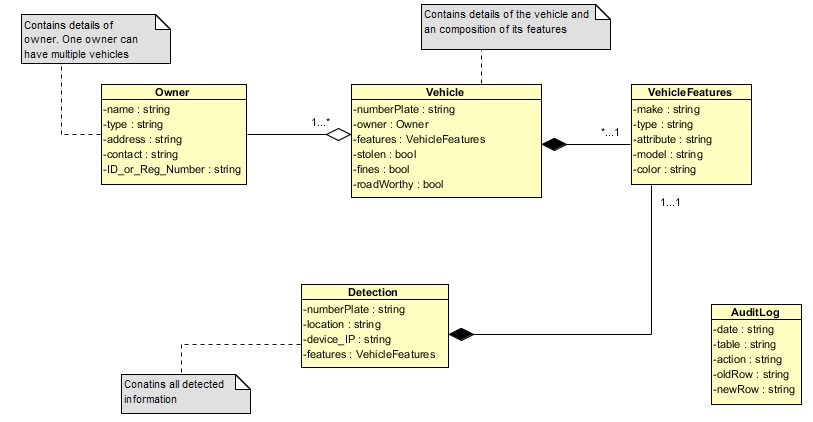
\includegraphics[width=6.25in, height=3.11in]{Pictures/CoreDomainObjects.jpg}
		                             \caption{Core Domain Objects}
		             		\end{figure}
               %\section{Glossary}
             
\end{document}


